\section{Result and Systematic Uncertainties}
\label{sec:syst}
\emph{In short: thirteen variants in four groups, fitted by both methods on the same candidates, give $0.0070$ (Bayesian) and $0.0072$ (Frequentist), dominated by the particle-identification requirement.}
The result depends on choices of the analysis that the data do not fix. They were varied one at a time in thirteen variants, fitted by both methods on exactly the same candidates and combined with the same rule. The variants fall in four groups: the \emph{window} (lower edge $5050$ and $5150\,\MeV$, upper edge $5450$ and $5700\,\MeV$), the \emph{background} model (single exponential, shape shared between the charges, charge-symmetric background $A_b=0$), the \emph{signal} model (Crystal Ball, $\mu$ and $\sigma$ per charge) and the \emph{preselection} ($\texttt{ProbK}>0.4$ and $0.6$, $\texttt{ProbPi}<0.4$ and $0.6$). When a variant changes the sample (window, preselection) the two samples are nested and part of the shift $\Delta=\Araw^{\mathrm{var}}-\Araw^{\mathrm{nom}}$ is a statistical fluctuation of expected size $\sigma_B=\sqrt{|\sigma_{\mathrm{var}}^2-\sigma_{\mathrm{nom}}^2|}$~\cite{barlow}, so the variant contributes only if $|\Delta|>\sigma_B$; a variant that the data reject (the single exponential) is excluded; the largest remaining $|\Delta|$ of each group is its uncertainty and the groups, being independent choices, are added in quadrature\appfig{sec:syst_tables}{Tables~\ref{tab:bayes_all} and~\ref{tab:syst}}.
The groups give $0.0014$ (window), $0.0037$ (background), $0.0002$ (signal) and $0.0058$ (preselection) in the Bayesian fit and $0.0014$, $0.0040$, $0.0006$ and $0.0058$ in the Frequentist one, for totals of $0.0070$ and $0.0072$; the two methods give the same shifts to within $\sim$$0.0005$. The \textbf{preselection} dominates, through the single variant $\texttt{ProbK}>0.6$ ($+0.0058$, $1.2\,\sigma_B$), which a scan of each cut in steps of $0.05$ shows to be a \emph{fluctuation}: on the tight side the shifts scatter around zero within $1.3\,\sigma_B$ without a trend, whereas loosening $\texttt{ProbK}$ moves $\Araw$ monotonically, as expected if misidentified decays not in the mass model enter the sample (Fig.~\ref{fig:pid_scan_body})\appref{app:syst_results}. The nominal requirement is therefore well placed and the preselection uncertainty conservative. The shifts of the thirteen variants are shown in Fig.~\ref{fig:syst_variants}, and the final result is
\begin{gather*}
\text{Bayesian:}\\ \Araw=-0.0443\pm0.0085\,(\text{stat})\pm0.0070\,(\text{syst}),\\[2pt]
\text{Frequentist:}\\ \Araw=-0.0441\pm0.0085\,(\text{stat})\pm0.0072\,(\text{syst}).
\end{gather*}

\begin{figure*}[!t]
\centering
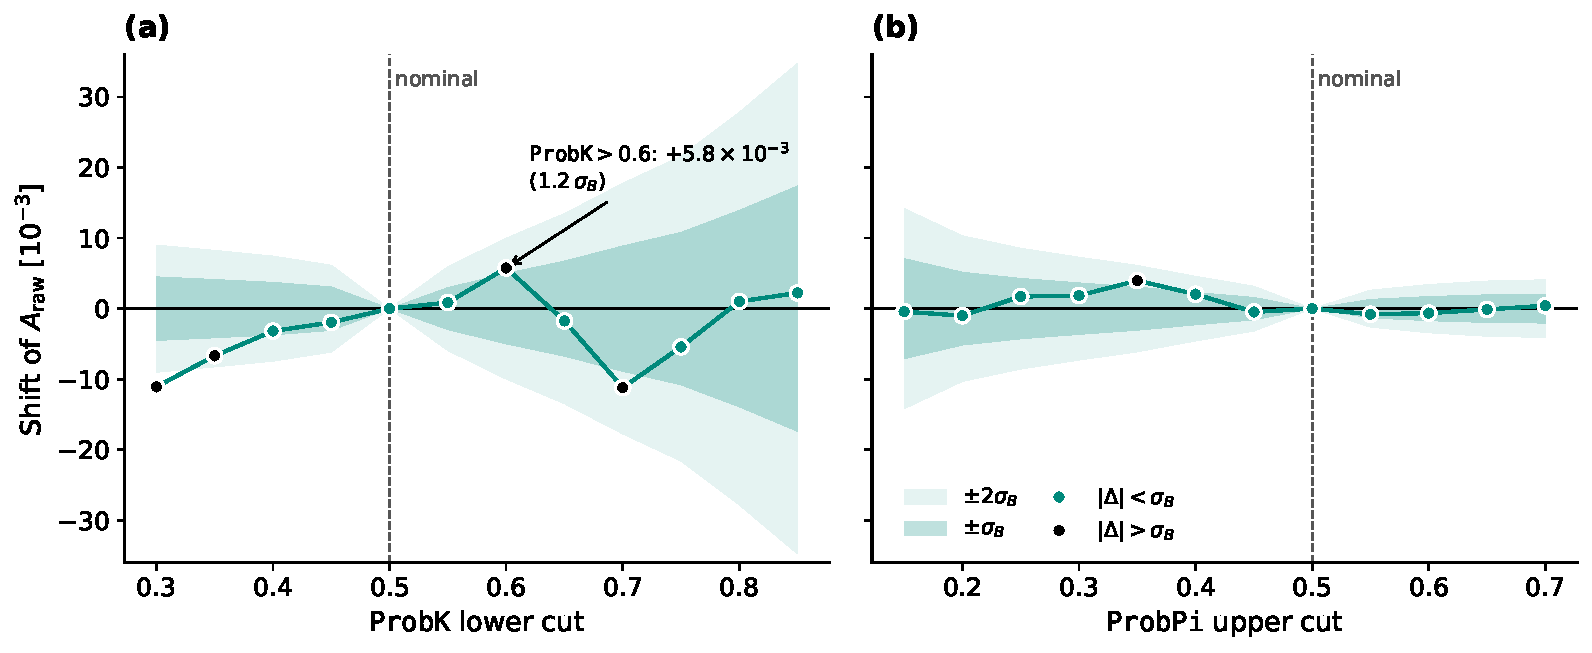
\includegraphics[width=0.80\textwidth]{figures/short_pid_scan.pdf}
\caption{Shift of $\Araw$ (Frequentist fit) as a function of (a) the $\mathtt{ProbK}$ lower cut and (b) the $\mathtt{ProbPi}$ upper cut, in steps of $0.05$, with the expected statistical spread of the nested sample ($\pm\sigma_B$ dark, $\pm2\sigma_B$ light; zero at the nominal cut, dash-dotted line). On the tight side of $\mathtt{ProbK}$ the points scatter around zero without trend and the pion requirement is flat; loosening $\mathtt{ProbK}$ moves $\Araw$ monotonically.}
\label{fig:pid_scan_body}
\end{figure*}

\begin{figure}[t]
\centering
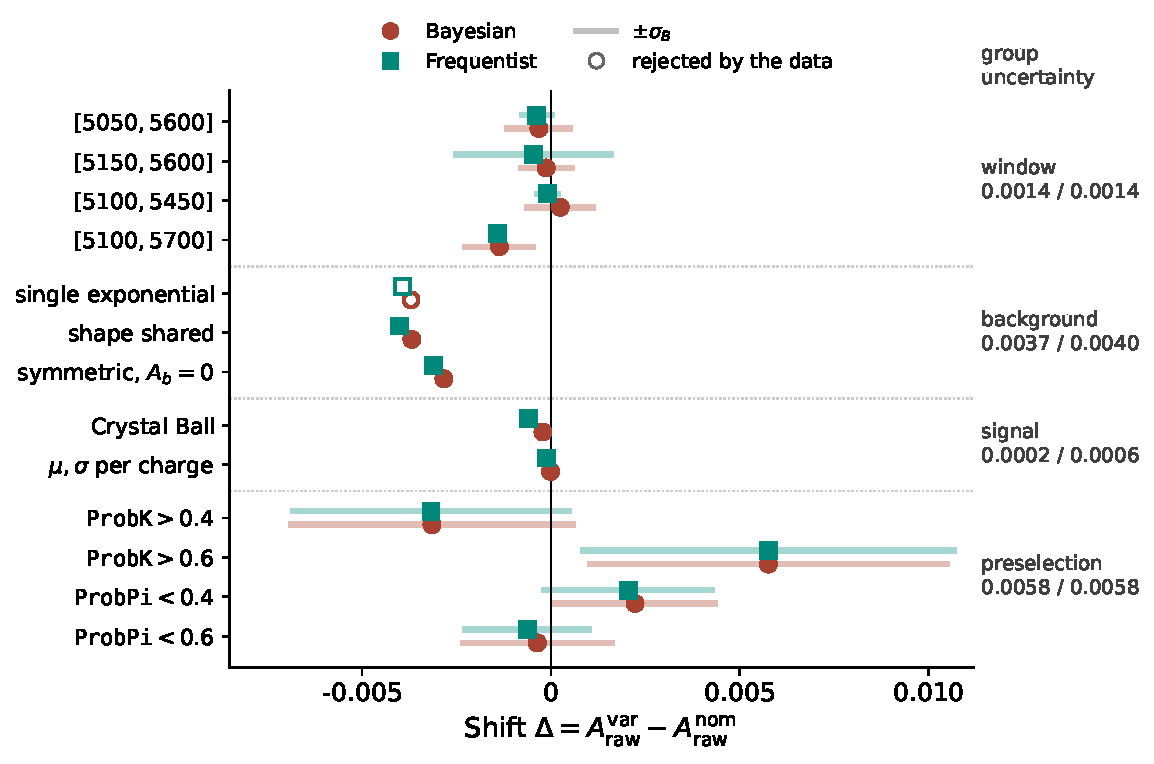
\includegraphics[width=\columnwidth]{figures/short_syst_variants.pdf}
\caption{Shift $\Delta$ of $\Araw$ for the thirteen variants of the analysis, in the Bayesian (circles) and Frequentist (squares) fits, with the expected statistical spread $\sigma_B$ of the variants that change the sample (bars); the open markers are the variant rejected by the data. On the right, the uncertainty of each group (Bayesian / Frequentist), its largest contributing shift.}
\label{fig:syst_variants}
\end{figure}

\subsection{Additional Results}
\emph{Checks.} The $\sigma_B$ rule is verified by bootstrap (the spread of the shift between a sample and its tighter subsample is $\sigma_B$). %and the grid scans of the Frequentist fit move $\Araw$ by at most $0.0126$ (PID cuts, smaller samples), $0.0048$ (window edges) and $6\times10^{-5}$ (signal region)\appfigs{sec:checks_barlow}{Fig.~\ref{fig:checks_barlow}}{sec:freq_stab_numbers}{Fig.~\ref{fig:freq_stability}}.
